101. $$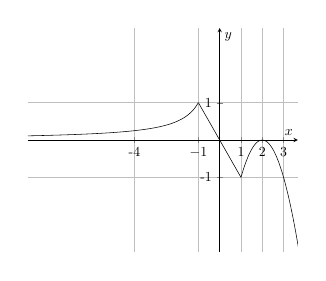
\begin{tikzpicture}[scale=0.5]
\begin{axis}[
    axis lines = middle,
    grid=major,
    legend pos={south west},
    xlabel = {$x$},
    %xlabel style={below right},
    ylabel = {$y$},
    ymin=-3,
    ymax=3,
    xtick={-4, -1, 1,2, 3, 4},
    xticklabels={-4, $\text{                  -1}$, 1,2, 3, 4},
    ytick={-1 , -4, 1},
    yticklabels={-1 , -4, 1},
                  ]
	\addplot[domain=-9:-1, samples=100, color=black] {-1/x};
    \addplot[domain=-1:1, samples=100, color=black] {-x};
    \addplot[domain=1:9, samples=100, color=black] {-x*x+4*x-4};
\end{axis}
\end{tikzpicture}$$
По графику определим ответ: $m\in(-1;0).$
\newpage
